\section{Testing the model}
Different steps need to be followed in order to test the Global View Model proposed over the multi-layer traffic workload model. First of all is necessary to test the mixture idle distribution and check if it efficiently describes the idle process. 

% JOHN: This "testing" consists of two tests, namely, testing the fitting and testing how it is related to the active time distribution, [i.e. the packet lengths]

\subsection{Mixture idle distribution}
As it has been explained before in this document, the mixture idle distribution of the semi-markovian model can be expressed as a combination of two distributions: Uniform distribution for $[0 < t < \alpha_{bk}]$ and a long-tail that can be approximated by a Truncated Generalized Pareto in $[t > \alpha_{bk}]$. This can be expressed as it is presented in (\ref{eq:Idle}).

In order to test this mixture distribution, we generated different tests with medium-load traffic. The user realization for these tests is represented in Figure \ref{fig:test_model_network}. Different traffic configurations has been used for the tests and the \acs{CDF} and PDF of the Idle distribution has been extracted. In Figure \ref{fig:cdf_globalview} is represented one of those tests.

% JOHN: In the text above, you can be more general. Do not refer now to Figures and results, just describe the test itself.

\begin{figure}
	\centering
	\includegraphics[scale=0.35]{images/results/GlobalView/test_model_network}
	\caption{Testing the mixture model - Users distribution}
	\label{fig:test_model_network}
\end{figure}

\begin{figure}[t]
	\centering
	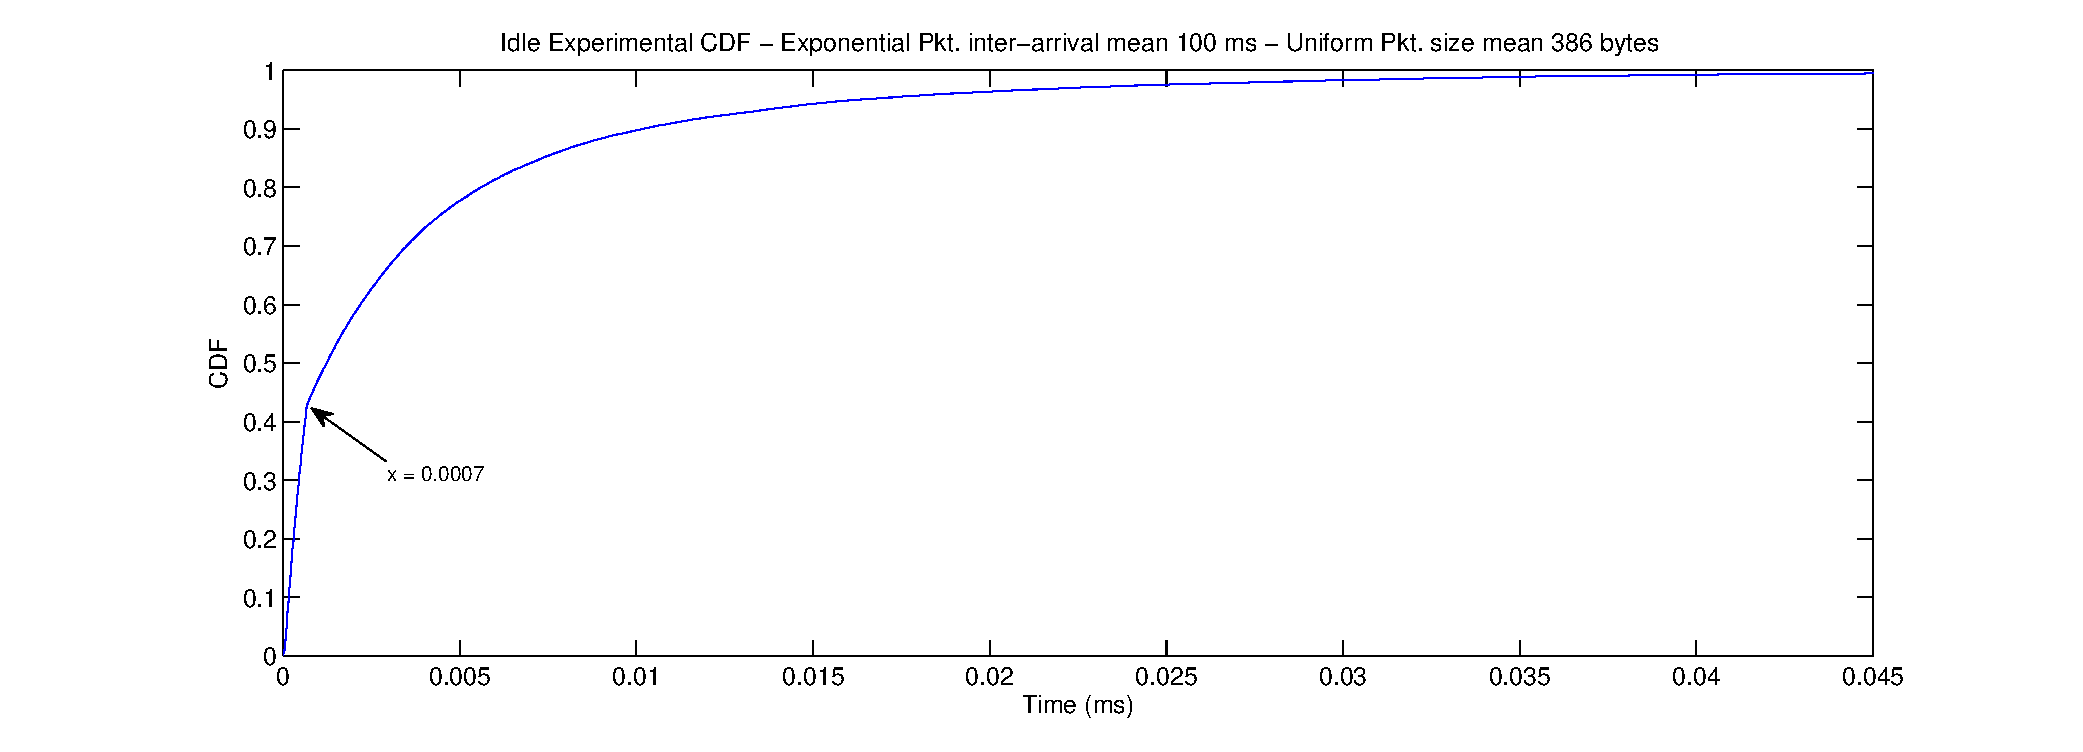
\includegraphics[scale=0.28, trim = 0mm 0mm 6mm 180mm, clip]{images/results/GlobalView/cdf_globalview}
	\caption{Idle distribution}
	\label{fig:cdf_globalview}
\end{figure}

From Figure \ref{fig:cdf_globalview} can be observed that there are two differentiated behaviors in the Idle \acs{CDF}: a part that follows an uniform distribution in the area of $[0 < t < \alpha_{bk}]$, and a long-tail in $[t > \alpha_{bk}]$. Then, this Idle distribution can be perfectly approximated by the proposed mixture idle distribution defined in (\ref{eq:Idle}).

% JOHN: Again, result discussion should not go in this section. If you want to show an illustrative example of the pdf, cdf of the mixture idle, just do it before, in the model description section.

\subsection{Idle - Active independency}
Another important claim of the proposed semi-markovian model is that the Idle and Active functions are independent, meaning that for the same Idle distribution, different Active distributions should not affect the performance of the Idle distribution of the model. In order to test this, it is necessary to configure the multi-layer traffic model as it is explained at the beginning of this chapter, changing just one configuration parameter for the distribution of each layer at a time. For this, the session and flow levels will be the same for all the tests\footnote{All the sessions will begin at 0, while the number of flows per user and its interarrival times will be always the same for all the tests.}. For the packet level, it is necessary to configure the interarrival times between packets and its size. The Idle distribution is affected by the interarrival times between packets. For the Active distribution, different random distribution models for the packet size will be used for the same Idle distribution. In Figure \ref{fig:cdf_composed} is represented one of the tests performed to test the Idle-Active independency. It can be observed that for the same Idle distribution (i.e. Exponential interarrival with 100 ms of mean) and different Active distributions with the same mean, the Idle function is not affected which supports the claim that both distributions are independent.

% JOHN: There is a bit of confusion here. The "claim" of the Markovian modeling is the well-known Markov property, i.e. the time periods spent in adjacent states [in time] are independent random variables. This is NOT tested here. At this point, we test whether the Active distribution changes affect the idle behavior. Somehow, we test the sensitivity of the idle distribution against different packetization processes. So this is what must go in this section, to make it clear. Again, try not to discuss results at this point, leaving everything for the end of the section.

\begin{figure}[t]
	\centering
	\includegraphics[scale=0.28, trim = 0mm 0mm 6mm 0mm, clip]{images/results/GlobalView/cdf_composed}
	\caption{Idle function behavior for different Active distributions}
	\label{fig:cdf_composed}
\end{figure}

On the other hand, if the same tests are repeated in the opposite way (fixing the Active function and using different Idle distributions) it can be observed how different Idle distributions affect the behavior of the Idle function. This is represented in Figures \ref{fig:cdf_exponential} and \ref{fig:cdf_idle_same_mean}.
% JOHN: This is a good example of how all sentences in this section should look like! You discuss the description of the experiments and the possible results out of them, but do not refer to them directly, here.

\begin{figure}[h]
	\centering
	\subfloat[]{
		\label{fig:cdf_exponential}
		\includegraphics[scale=0.28, trim = 0mm 0mm 6mm 180mm, clip]{images/results/GlobalView/cdf_exponential}
	}
	\\
	\subfloat[]{
		\label{fig:cdf_idle_same_mean}
		\includegraphics[scale=0.28, trim = 0mm 0mm 6mm 180mm, clip]{images/results/GlobalView/cdf_idle_same_mean}
	}
	\caption{Idle function behavior for different Idle distributions}
	\label{fig:cdf_p}
\end{figure}

In Figure \ref{fig:cdf_exponential} an Uniform Packet size with mean 1550 bytes had been used all the tests while we used an Exponential distribution with different mean times for the interarrival packet time. It can be observed how the proportionality between the mean values of the Idle distribution affect also proportionally the Idle function. A low mean value means a higher load in the network and shorter Idle times.

In Figure \ref{fig:cdf_idle_same_mean} is represented the same case with an Uniform Packet size with mean 1550 bytes and different random distributions with the same mean for the Idle distribution. It can be observed that the Idle function is almost the same for different random distribution if they have the same mean.

% JOHN: Overall, as a general hint for this section: You could do the following: Introduce the tests and motivation at one subsection and ALL these results at the second one. 

